% !TeX spellcheck = en_US
\documentclass{IEEEtran}

\usepackage{graphicx}
\usepackage{amsmath}
\usepackage[numbers]{natbib}

\begin{document}

\title{Multi-Source Emotion Tagging for Online News}

\DeclareRobustCommand*{\IEEEauthorrefmark}[1]{%
  \raisebox{0pt}[0pt][0pt]{\textsuperscript{\footnotesize\ensuremath{#1}}}}

\title{Multi-Source Emotion Tagging for Online News}
\author{\IEEEauthorblockN{Li Yu\IEEEauthorrefmark{1}, Zhifan Yang\IEEEauthorrefmark{1}, Peng Nie\IEEEauthorrefmark{2}, Xue Zhao\IEEEauthorrefmark{1}, Ying Zhang$^*$\thanks{* Corresponding Author}\IEEEauthorrefmark{1}\IEEEauthorrefmark{2}\\}
\IEEEauthorblockA{\IEEEauthorrefmark{1}College of Computer and Control Engineering, Nankai University \\}
\IEEEauthorblockA{\IEEEauthorrefmark{2}College of Software, Nankai University}\\
}



\maketitle


\begin{abstract}
With the rapid growth of social media and online news services, users nowadays can respond to online news by rating subjective emotions such as happiness, surprise or anger actively. Once the user ratings is over a certain range, it begins to show up a tendency of what most people think and feel, which can help us understand the preferences and perspectives of most users, and help news providers to provide users with more positive news. Thus it has become a pregnant research problem to tag emotion automatically.
This paper tackles the task of emotion tagging for online news with multi-source including news article and comment, as emotion is not only tagged after reading news article, but also can be incorporated in comment with what they feel. In this paper, a novel classification model are proposed with two layer logistic regression. The new approach get outputs from basic classifiers and combine them in a new classifier, making a more accurate prediction when compared with a single source method. An extensive set of experimental results on a real dataset from a popular online news service demonstrate the effectiveness of the proposed approach. 
\end{abstract}

\begin{keywords}
Sentiment Tagging; Online News; Meta Classification; Multiple Source
\end{keywords}

\section{Introduction}
With the explosive growth of the Internet, a large number of social media have been produced and its influence continues to increase. Online news is an important form that attracts millions of users to read and express their feelings among kinds of social media. Users often express their subjective emotions such as sadness, surprise and happiness by rating emotion tags after reading news. Figure \ref{figure:sinavotes} shows an example emotion tagging from a popular Chinese news website (i.e. The Society Channel of Sina News\footnote{http://news.sina.com.cn/society/}).
\vspace{-10pt}
\begin{figure} [!h]
\centering
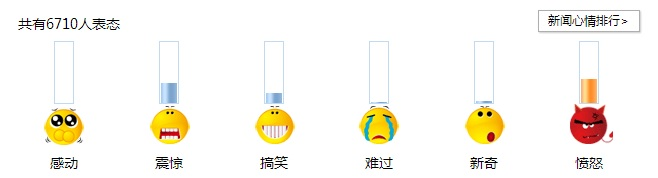
\includegraphics[width=1\linewidth]{sinavotes.jpg}
\caption{An example of emotions and user ratings}
\label{figure:sinavotes}
\end{figure}

Sentiment analysis of online documents such as news articles, blogs and microblogs has received increasing attention in recent years and it is a challenging research problem to do emotion tagging for online news automatically. Naturally, we classify news to each emotion tags based on the content of news article, as the news article is what they read and directly influences their emotion rating. What is more, an increasing number of social news websites provide comment service where users can share what they feel after reading news articles. Thus news comment provide another significant source for emotion tagging.

Sentiment classification model generally fall into two categories, generative models and discriminative models. As the second one has attractive theoretical properties, we adopt logistic regression as our basic method. Two basic classifiers are built to get the outputs of single source. Through utilizing the outputs of multiple sources including news article and comment, we propose a novel approach by two-layer prediction. Since different source has its own effect on emotion prediction in different situations, we match different source with different weighting parameters, making it more adaptable.

In addition, we provide an experiment on a real dataset after detailed analysis. In the experiment, we introduce the experimental environment and give the statistic data on dataset. Our proposed approach with multi-source are compared with basic approaches with single source in different size of dataset. Finally we verify the necessity of multi-source for emotion tagging and the effectiveness of the proposed model after experimenting on the dataset, society channel of Sina News .In particular, the proposed model has shown better performance on Sina dataset than baselines. The robustness of the proposed discriminative meta classification models is evaluated with different sizes of dataset. 

%The contribution of this paper can be listed as followed,
%\begin{itemize}
%\item Our work consider the difference between different sources and give separated weighting parameters to each source.
%\item Our work consider to be generalized without the impact of language.
%\item Our work has been approved to be effective on Sina dataset thus can be applied on other multi-source applications.
%\end{itemize}

The rest of the paper is organized as follows. In Section \ref{section:RelatedWork}, we review the state of the art on emotion tagging and make discussions regarding the difference between our work and previous work. In Section \ref{section:Method}, we propose our novel method with two layers. The experimental results are presented and discussed in Section \ref{section:Experiments}. Conclusions and future work are given in the last section \ref{section:conclusion}.

\section{Related Work}
\label{section:RelatedWork}

The Task of emotion tagging is to give an emotion label to text content. Early work in \citet{ekman1992argument} defined six basic emotion labels: happiness, sadness, anger, fear, surprise and disgust, which laying a good foundation in some existing work on emotion tagging including \citet{liu2003model, das2009word, das2010sentence, aman2008using}.
Specifically, \citet{liu2003model} used an ensemble of rule-based affect models to classify sentences into six basic emotion labels. Another kind of methods based on supervised learning considering the problem as text categorization or analogous to topic classification \citet{alm2005emotions} has also gone a long way. Along the way of this kind of method, \citet{das2009word, das2010sentence} used Naive Bayes and Support Vector Machines based on some online dictionary. \citet{aman2008using} proposed a method of building an dictionary derived from the \textit{Roget Thesaurus} \citet{roget1852}.

In addition, \citet{yang2007emotion} trained SVM model to investigate the emotion classification of web blog. Another work \citet{yang2007building} used Yahoo Kimo Blog corpora to build emotion dictionary. By considering the relationships between words in a sentences, \citet{neviarouskaya2007narrowing} proposed a syntactical approach to recognition emotion automatically. \citet{mishne2006capturing} used several supervised and unsupervised machine learning techniques on blog data for comparative evaluation. \citet{binali2012emotion} compared various text-based emotion detection techniques.

%The 4th International Workshop on Semantic Evaluations in 2007 organized an evaluation campaign on Semeval Task for ``Affective Text" (Task 14) \footnote{http://nlp.cs.swarthmore.edu/semeval/tasks/task14/summary.shtml}. The main task is the emotion classification of news headlines downloaded from some well-known news web sites(i.e. New York Times, CNN, and BBC News), as well as from the Google News search engine with Ekman's six emotion labels. Several participants experimented various techniques for the task. \cite{chaumartin2007upar7} developed a rule-based linguistic system by using a set of lexical resources. \cite{kozareva2007ua} gathered statistics from three commercial search engines to determine the kind and the amount of emotion in each headline. Emotion score are obtained by using Pointwise Mutual Information. \cite{katz2007swat} used a combination of four classifiers including Naive Bayes, nearest neighbor cosine, decision lists, and latent semantic analysis. Synonym expansion on the emotion label words is also performed, using the \textit{Roget Thesaurus} \cite{roget1852}. Based on the Semeval corpus, \cite{strapparava2008learning} conducted comparative evaluations of several knowledge-based and corpus-based methods.

Moreover,\citet{bao2009joint, bao2011mining} proposed a topic model by augmenting latent Dirichlet allocation (LDA) with an intermediate layer for emotion modeling whose experiments were conducted on a dataset collected from the news website Sina. \citet{lin2007emotions, lin2008emotion} studied the classification of news articles into emotions that they invoke on their readers instead of the authors.
On the other hand, people try to do emotion tagging for online news comments in \citet{zhang2012emotion, ZhangZSLWY14}, which uses a fixed combination strategy to merge heterogeneous information sources. In this paper, we use a novel model with multi-source on a real-world dataset to evaluate the effectiveness of the proposed approach.


\section{Multi-Source Emotion Tagging}
\label{section:Method}
In this section, a novel method named Multi-Source Emotion Tagging for online news is proposed based on combining multiple source' results. We firstly define our research problem in section \ref{section:Definition}. Then we apply basic logistic regression on news article and comment in section \ref{section:newscontent} and \ref{section:newscomment}. Finally we propose the approach of two-layers for the scenario combining multi-source prediction results to do a second prediction in section \ref{section:key}.

\vspace{-10pt}
\subsection{Problem Definition}
\label{section:Definition}
Here we set the definition of research problem for online news. We have a collection of comment $\mathcal{C}$ which are made by users after reading online news articles $\mathcal{D}$. All features in news article and comment are from $\mathcal{V}$, an emotion word dictionary.
We also predefined the emotion set $\mathcal{E} = \{e_{k}\}(k=1,\ldots,K)$ from which we select emotion for the news. The $i_{th}$ news article $d_i$ is associated with a user-generated comment combination $c_i$ over each emotion $e_k$. Each news article $d$ has an emotion tagging variable ${t} = \{t_{k}\}$ denoting how each emotion the reader expresses aftering reading news. As a result, there exists $\sum_{k=1}^{K}{t_{k}} = 1$.

We take the problem of emotion tagging for online news into a multi-class classification that classifies news into different emotion tags. We adopt multi-source including the news article and its' comment combination to achieve the goal.

\subsection{Emotion Tagging with News Article}
\label{section:newscontent}
%Sentiment classification model generally fall into two categories, generative models and discriminative models. The discriminative models have attractive theoretical properties. Thus we adopt logistic regression, one of the discriminative probabilistic models to solve the problem of emotion tagging with news article.

Formally, given the $i_{th}$ news article $d_i$, we denote the conditional probability that the news will be tagged as a predefined emotion $e_k$ by a logistic regression as $\xi_{ik}$. The parametric form of $\xi_{ik}$ can be expressed as follows in terms of soft-max function over a linear function of features,

\vspace{-7pt}
\begin{equation}
\label{eq:pc}
{\xi _{ik}} = P({e_k}|{d_i}) = \frac{{\exp ({\alpha _k}{s_i})}}{{\sum\limits_{k = 1}^K {\exp } ({\alpha _k}{s_i})}}\
\end{equation}
\vspace{-7pt}

Here $s_i$ represents the feature vector of news $d_i$, $\alpha_{k}$ denotes the combination parameters for each term with emotion $e_k$. Then we need to estimate the parameter $\alpha$ by maximizing the likelihood function as follow,

\vspace{-7pt}
\begin{equation}
\mathop {\max \;}\limits_\alpha  \prod\limits_{{d_i} \in {\cal D}} {\prod\limits_{k = 1}^K {{\xi _{ik}}^{{t_{ik}}}} }
\end{equation}
\vspace{-7pt}

For the sake of simplicity, we usually minimize the negative log-likelihood function with L2 (i.e., ridge) regularization, and we call it the loss function as below,

\vspace{-7pt}
\begin{eqnarray}
\mathcal{L}(\alpha)  =  -\sum_{d_i \in \mathcal{D}}\sum_{k=1}^{K}t_{ik}\log{\xi_{ik}}+\lambda{R(\alpha)}
\end{eqnarray}
\vspace{-7pt}

Here L2 regularization term can be written with the following notation,

\vspace{-7pt}
\begin{equation}
R(\alpha) = \|\alpha\|_2^2 = \sum_{k=1}^{K}\sum_{v_j \in \mathcal{V}}{\alpha^2_{kj}}
\end{equation}
\vspace{-7pt}

Finally, the loss function can be expressed as below,

\vspace{-10pt}
\begin{eqnarray}
{\cal L}(\alpha ) &=&  - \sum\limits_{{d_i} \in {\cal D}} {\sum\limits_{k = 1}^K {{t_{ik}}} } ({\alpha _k}{s_i} - \log (\sum\limits_{r = 1}^K {\exp } ({\alpha _r}{s_i})))\\ &+& \lambda \sum\limits_{k = 1}^K {\sum\limits_{{v_j} \in {\cal V}} {\alpha _{kj}^2} } \nonumber
\end{eqnarray}
\vspace{-14pt}

\subsection{Emotion Tagging with Comment}
\label{section:newscomment}
Similar as section \ref{section:newscontent}, we describe the emotion tagging with comment in this section.  In the $i_{th}$ news, we combine the top news comment together as $c_i$. It will be tagged as a predefined emotion $e_k$ by the Equation \ref{eq:pc2}, referred as $\eta_{ik}$.

\vspace{-5pt}
\begin{equation}
\label{eq:pc2}
{\eta _{ik}} = P({e_k}|{c_i}) = \frac{{\exp ({\theta _k}{x_i})}}{{\sum\limits_{k = 1}^K {\exp } ({\theta _k}{x_i})}}
\end{equation}
\vspace{-7pt}

The combination parameters $\theta_{k}$ can be estimated by minimizing the following loss function with L2 (i.e., ridge) regularization in the training set.

\vspace{-5pt}
\begin{eqnarray}
{\cal L}(\theta ) &=&  - \sum\limits_{{d_i} \in {\cal C}} {\sum\limits_{k = 1}^K {{t_{ik}}} } \log {\eta _{ik}} + \lambda R(\theta )\\
&=&  - \sum\limits_{{c_i} \in {\cal C}} {\sum\limits_{k = 1}^K {{t_{ik}}} } ({\theta _k}{x_i} - \log (\sum\limits_{r = 1}^K {\exp } ({\theta _r}{x_i}))) \nonumber \\
&+& \lambda \sum\limits_{k = 1}^K {\sum\limits_{{v_j} \in {\cal V}} {\theta _{kj}^2} } \nonumber
\end{eqnarray}
\vspace{-5pt}

%\begin{equation}
%\begin{split}
%&\mathcal{L}(\theta)=-\sum_{d_i \in %\mathcal{C}}\sum_{k=1}^{K}t_{ik}\log{\eta_{ik}}+\lambda{R(\theta)}\\
%&=-\sum_{c_i \in %\mathcal{C}}\sum_{k=1}^{K}t_{ik}\log{\frac{\exp(\theta_{k}^{T}x_{i})} %{\sum_{r=1}^{K}\exp(\theta_{r}^{T}x_{i})}}+\lambda{\sum_{k=1}^{K}\sum_%{v_j \in \mathcal{V}}{\theta^2_{kj}}}
%\end{split}
%\end{equation}

Here, $x_{i}$ represents the feature vector of news comment and $\eta_{ik}$ denotes the probability that the news comments $c_i$ will be tagged as an emotion $e_k$.

\vspace{-10pt}
\subsection{Multi-Source Emotion Tagging}
\label{section:key}
As different information source can bring different insight on emotion tagging, our new proposed method named multi-source emotion tagging utilizing multiple sources' prediction outputs to gain more accurate result.
Firstly, we do single source emotion tagging training as section \ref{section:newscomment} and \ref{section:newscontent}. Then we combine the two outputs and a constant bias as a new feature vector. Let $\psi_i$ denote the combined news features, i.e. $\psi_i = \{\xi_{i1},\xi_{i2},...,\xi_{iK},\eta_{i1},\eta_{i2},...,\eta_{iK},1\}$,we train $\psi_i$ in the train set making a two-layer training approach. Formally, the probability that emotion $e_k$ will be assigned to the $i_{th}$ news which can be estimated as below,

\vspace{-7pt}
\begin{equation}
{\mu _i} = \frac{{\exp ({\omega _k}{\psi _i})}}{{\sum\limits_{k = 1}^K {\exp } ({\omega _k}{\psi _i})}}
\end{equation}
\vspace{-7pt}

where $\omega _k$ denote the combination parameters for the multiple sources and the extra bias. These parameters can be determined by maximizing the following loss function.

\vspace{-7pt}
\begin{eqnarray}
{\cal L}(\omega ) &=& \sum\limits_{{c_i} \in {\cal C}} {\sum\limits_{k = 1}^K {{t_{ik}}} } \log {\mu _i}\\
&=& \sum\limits_{{c_i} \in {\cal C}} {\sum\limits_{k = 1}^K {{t_{ik}}} } ({\omega _k}{\psi _i} - \log (\sum\limits_{r = 1}^K {\exp } ({\omega _r}{\psi _i})))\nonumber
\end{eqnarray}
\vspace{-7pt}

Here, $\mu _i$ denotes the probability that the $i_{th}$ news will be tagged as an emotion $e_k$. 

\vspace{-10pt}
\section{Experiments}
\label{section:Experiments}
In this section, we firstly introduce our datasets. Then we describe experiments on real labeled datasets from the society channel of Sina website. Finally we compare the result on our method and single source baseline.

\vspace{-10pt}
\subsection{Datasets}
Web crawler have downloaded most-viewed news article, its matching comment and its user ratings from Society channel of Sina News, one of the largest news providers in China, starting from 2014/5/1 and ending with 2015/5/1. Since we have not find any user rating in English web service, we decide to use Sina dataset alone. However, our novel model is language independent. Among the $i_{th}$ news in Society channel of Sina News, we set a threshold of 20 to the user ratings and take its top 20 comment as collection $c_i$. Finally, we get 6821 news with its matching comment and ratings. Table \ref{tab:statdataset} gives detailed statistics of the dataset.

\begin{table}[!h]
\centering
\caption{The statistics of labeled news on Society Channel of Sina News}
\begin{tabular}{c c c}
\hline
Category & Count & Proportion\\
\hline
Touched & 1281 & 18.78\%\\
Shocked & 365 & 5.35\%\\
Amused & 1519 & 22.27\%\\
Sad & 940 & 13.78\%\\
Surprised & 165 & 2.42\%\\
Angry & 2551 & 37.40\%\\
Total & 6821 & \\
\hline
\end{tabular}
\label{tab:statdataset}
\end{table}

%Text content like news article and comment are segmented to words by ICTCLAS \citet{zhang2003hhmm} and emotion words among them is chosen to be the terms, as these terms are more likely to convey the emotion from users. In our text-based classifier, we utilize the emotion terms frequency(tf) in the content of documents as features.

\subsection{Evaluation Metrics}
We adopt two measures including Mean Reciprocal Rank ($MRR$) and Accuracy ($Accu@n$) with a 10-fold cross validation.
\vspace{-5pt}
\begin{enumerate}
\item Mean Reciprocal Rank ($MRR$) \\
Given a text content $T$, let ${rank_i}$ denote the position of its truth emotion $\overline{e}_i$ in the predicted emotion ranking list $\mathcal{E}_i$, MRR of the collection will be expressed as,
\vspace{-5pt}
\begin{equation}
MRR = \frac{1}{N}\sum_{i=1}^N \frac{1}{rank_i}
\end{equation}
\vspace{-5pt}
\item Accuracy ($Accu@m$)\\
Given a text content $T$, its truth emotion $\overline{e}_i$ and predicted emotion set $\mathcal{E}_i@{m}$ including $m$ top ranked emotions, $accu_i@m$ is defined as,

\vspace{-5pt}
\begin{equation} 
\label {eq:Accu}
accu_i@m = \left\{
\begin{array}{ll}
1, & \overline{e}_i \in \mathcal{E}_i@{m} \\
0, & \overline{e}_i \notin \mathcal{E}_i@{m}
\end{array}
\right.
\end{equation}
\vspace{-5pt}

Thus, $Accu@m$ for the entire collection  $\{T_i\} (i=1,\ldots, N)$ is:

\vspace{-10pt}
\begin{equation}
Accu@m = \frac{1}{N}\sum_{i=1}^N accu_i@m
\end{equation}
\vspace{-10pt}

where $N$ is the number of content in the dataset.
\vspace{-5pt}
\end{enumerate}

\subsection{Experimental Methods}

The following three methods are compared:
\begin{itemize}

%\vspace{3pt}
\item \textbf{News article Logistic Regression(NLR)}
This approach is mentioned in section \ref{section:newscontent} and based on logistic regression with the source of news article.
%\vspace{3pt}
\item \textbf{Comment Logistic Regression(CLR)}
This approach is mentioned in section \ref{section:newscomment} and based on logistic regression with the source of news comment.
%\vspace{3pt}
\item  \textbf{Multi-Source Logistic Regression(MSLR)}
This approach is proposed in section \ref{section:key} and based on a two-layers multi-source logistic regression.

\end{itemize}


\subsection{Experimental Results}


Table \ref{tab:accu@n} present the evaluation results in Accu@n(n=1,2,3) on each method and The $\dagger$ symbols indicate statistical significance with p-value $<$ 0.001 with each model in comparison to NLR and CLR respectively. Through this table, our proposed method achieves the best result in Accu@n(n=1,2,3) and shows the robustness of the proposed discriminative meta classification models.
%\vspace{-5pt}
\begin{table}[!h]
	\centering
	\caption{Results of three models on society channel of Sina News.}
	\begin{tabular}{l l l l}
		\hline
		Methods & Accu@1 & Accu@2 & Accu@3\\
		\hline
		MSLR & 0.5831 $\dagger$ & 0.7738$\dagger$ & 0.8642$\dagger$ \\
		NLR & 0.5640 & 0.7518 & 0.8466 \\
		CLR & 0.5594 & 0.7433 & 0.8406 \\
		\hline
	\end{tabular}
	\label{tab:accu@n}
\end{table}
%\vspace{-5pt}


Experiment also explore the influence of the data size to our proposed method and two baselines. 1/3, 2/3 and 3/3 of dataset have been selected randomly and repeated 100 times to observe the impact of dataset size.
The MRR and Accu@1 results of the three models in different sizes dataset are plotted in Figure \ref{figure:resultaccu} and \ref{figure:resultmrr}. This shows that more training data will bring more accurate prediction results to all models. In addition, NLR predicts better than CLR and our two layer method MSLR predicts better than all baselines.

\begin{figure}[!h]
\centering
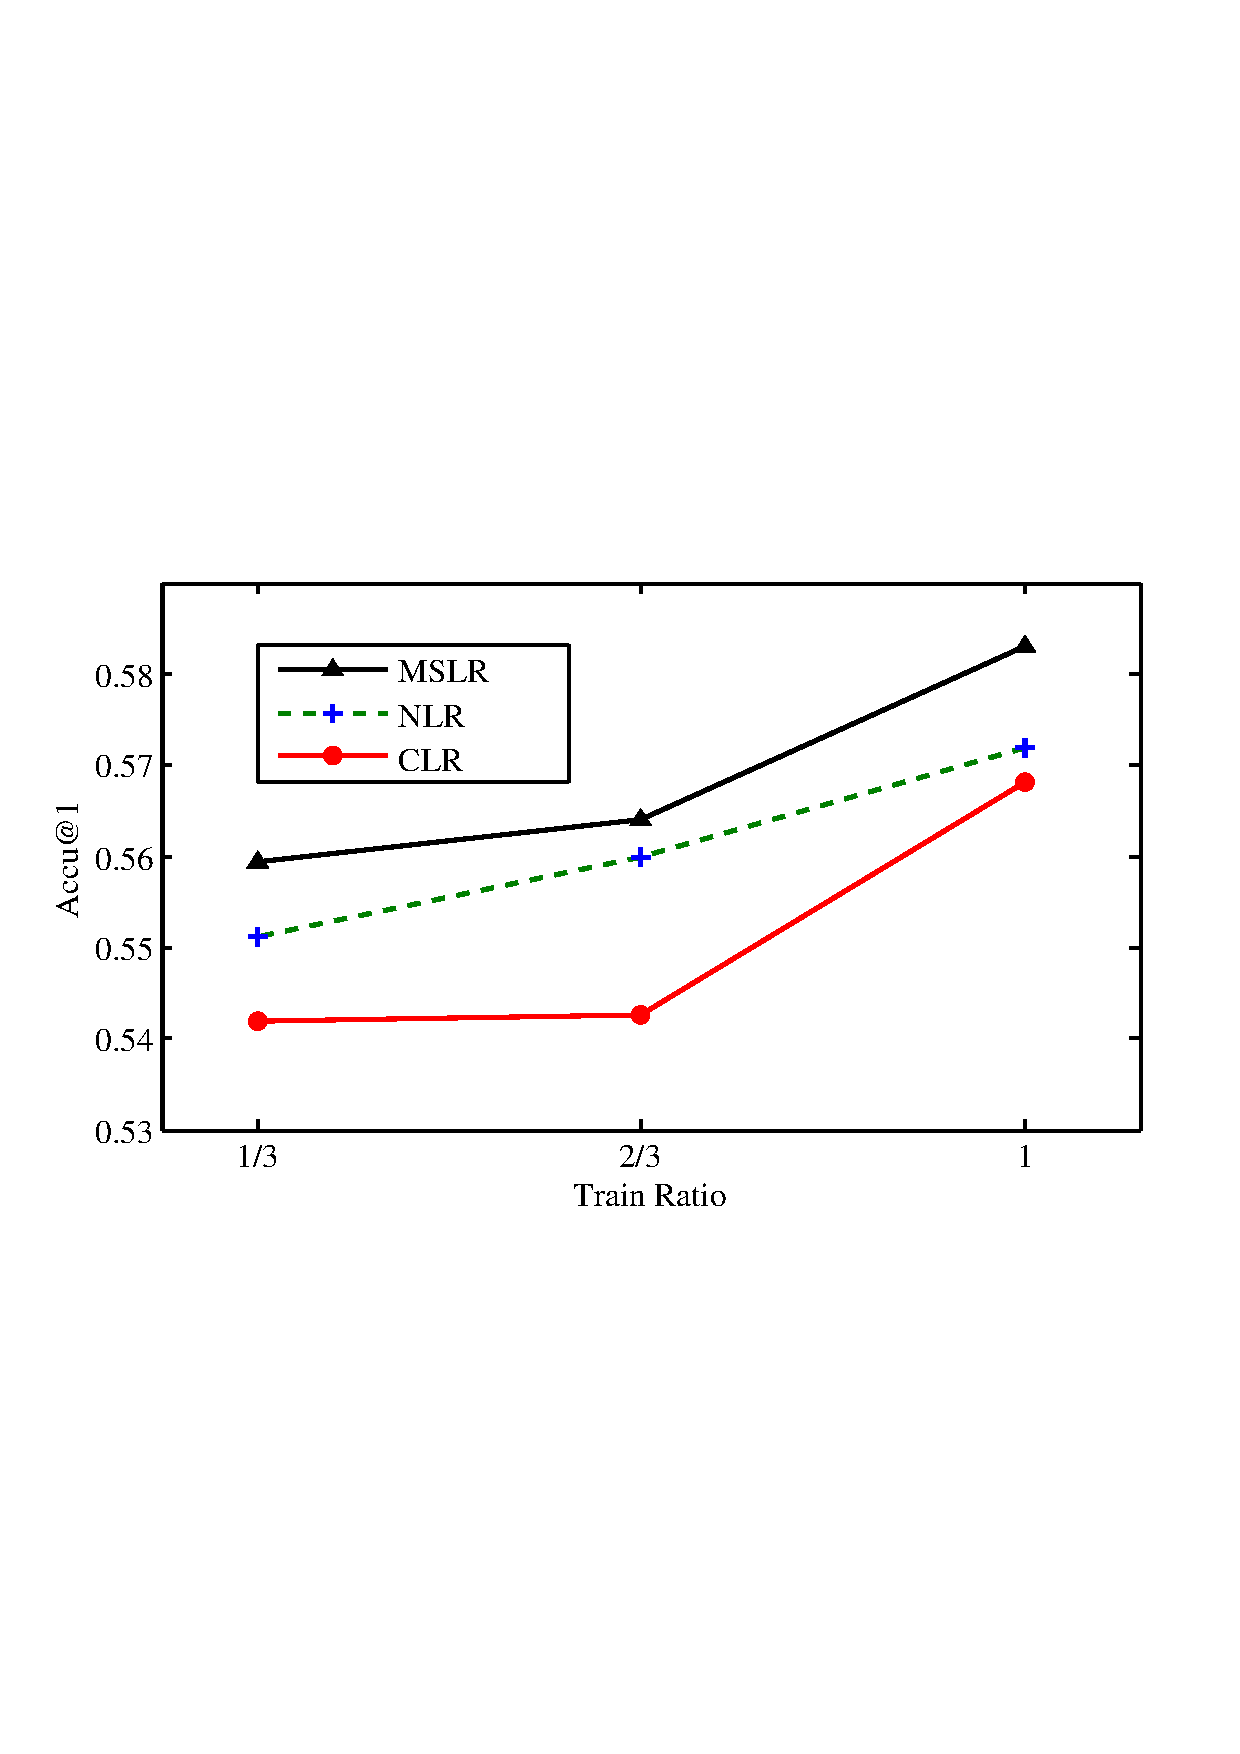
\includegraphics[width=1\linewidth,trim=0 240 0 280,clip]{Accu.pdf}
\vspace{-8pt}
\caption{The $Accu@1$ results on three models in different sizes of Sina dataset}
\label{figure:resultaccu}
\end{figure}
%\vspace{-5pt}
\begin{figure}[!h]
\centering
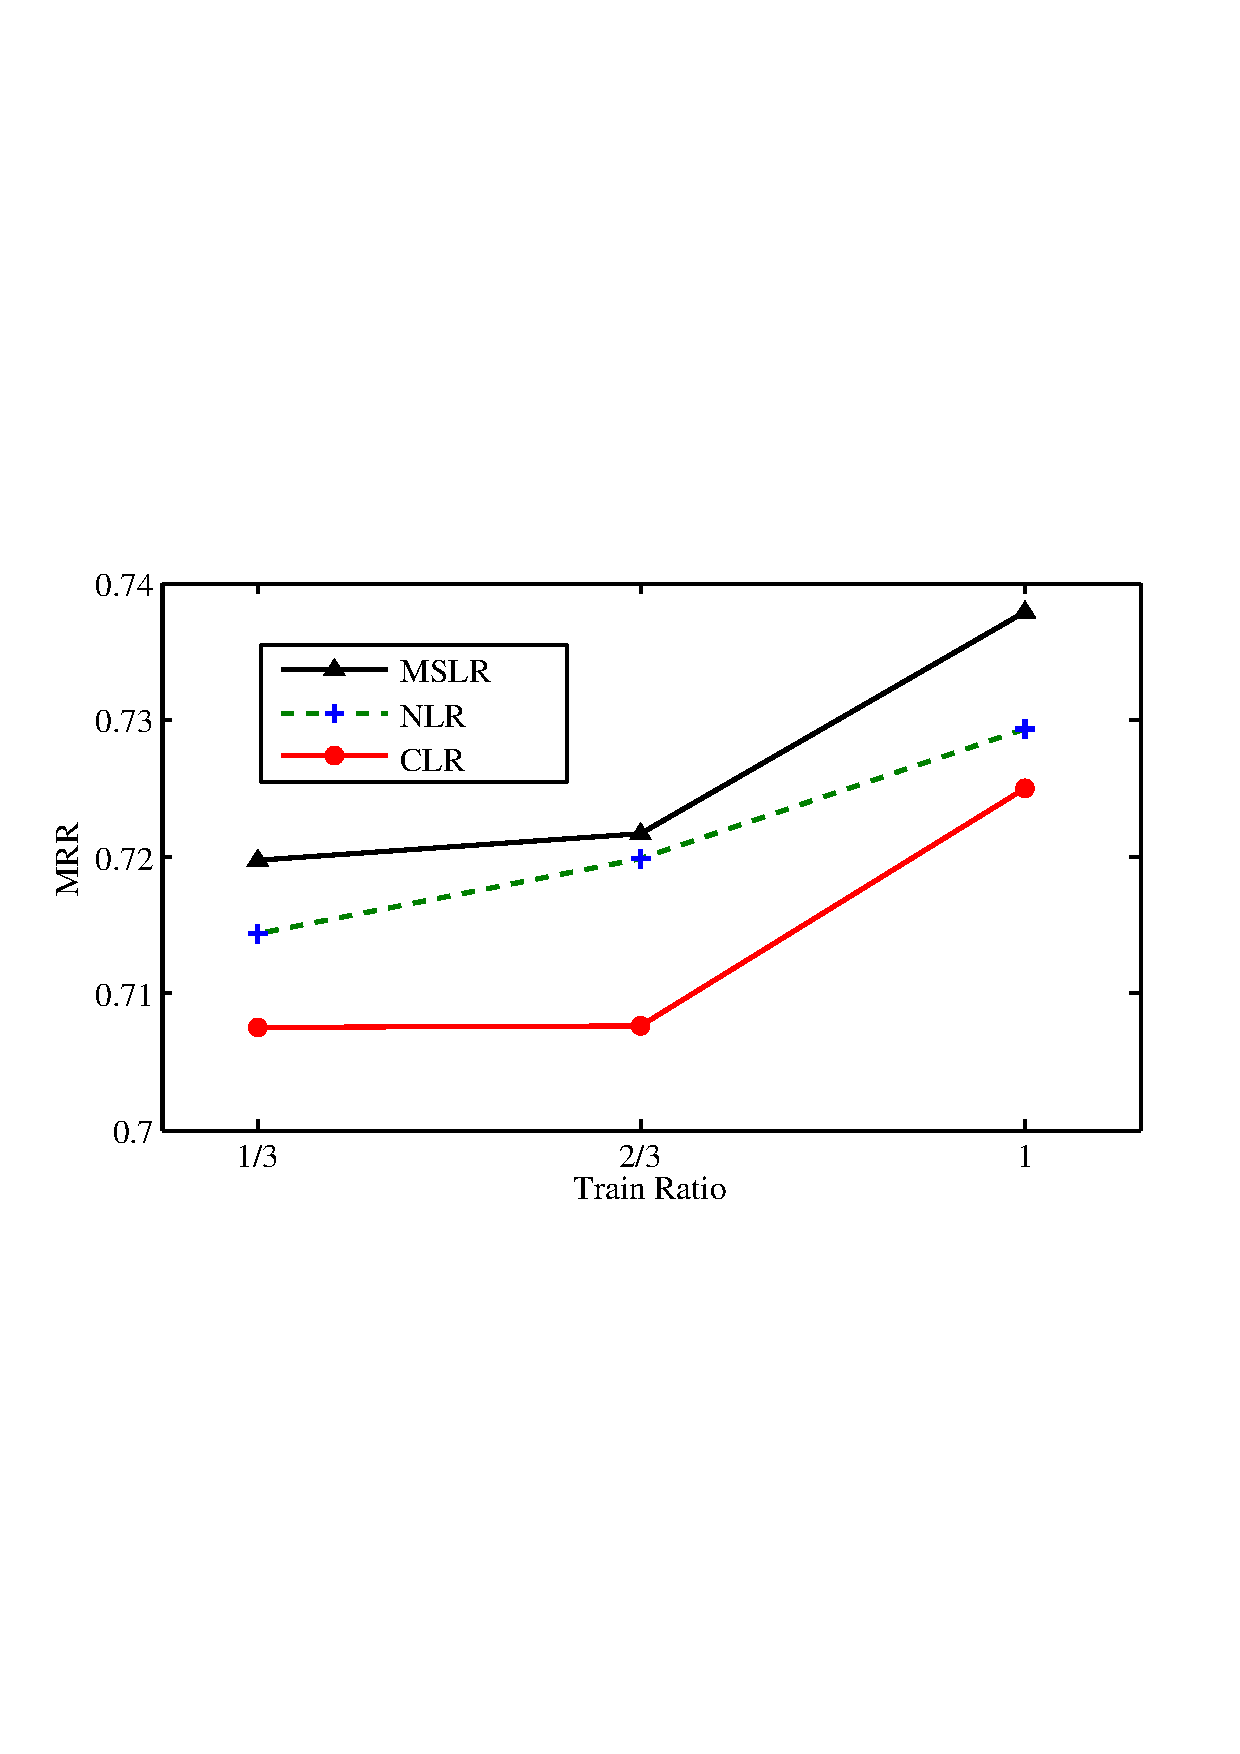
\includegraphics[width=1\linewidth,trim=0 240 0 280,clip]{MRR.pdf}
\vspace{-8pt}
\caption{The $MRR$ results on three models in different sizes of Sina dataset}
\label{figure:resultmrr}
\end{figure}
%\vspace{-10pt}

\section{Conclusion and Future Work}
\label{section:conclusion}
The emergence of online news and social media has promoted the rapid evolution of global conversation. Emotion tagging is a new problem need to be solved. This paper focuses on emotion tagging for online news.
We propose a meta classification model by treating emotion tagging for online news as second layer combination problem. Our two-layer method has provided a convenient way to combine multi-source information in one model. Empirical experiments have been conducted on the Sina datasets to show the effectiveness of the proposed probabilistic models by emotion tagging for online news.

This paper is an initial step to the emotion tagging research area. First of all, we plan to extend the work to the collection of online news. In addition, various types of relational information may be available on social media, such as user social network, users tagging news, users voting for comments and so on. The information can be utilized to improve emotion tagging and may lead to better prediction experience on social media. Moreover, it is worthwhile to exploring the emotion dictionary and emotion feature selection.

\section{Acknowledgment}
%\scriptsize
%The authors would like to thank the reviewers and the editors for their constructive suggestions.
This work is partially supported by National Natural Science Foundation of China under Grant No. 61402243, and Tianjin Municipal Science and Technology Commission under Grant No. 13ZCZDGX02200, 13ZCZDGX01098, and 14JCQNJC00200. This work is also partially supported by the Fundamental Research Funds for the Central Universities of China.
%This work is partially supported by National Natural Science Foundation of China under Grant No. 61402243, and Tianjin Municipal Science and Technology Commission under Grant No. 13ZCZDGX02200, 13ZCZDGX01098 and 14JCQNJC00200. This work is also partially supported by the Fundamental Research Funds for the Central Universities of China.

\scriptsize
\bibliographystyle{plainnat}
\bibliography{myref}
\end{document}
